\section{Поток и циркуляция магнитного поля. Дифференциальная и интегральная
форма уравнений магнитостатики. Граничные условия.}

\subsection*{Поток и циркуляция магнитного поля и Дифференциальная и интегральная
форма уравнений магнитостатики}

\begin{center}
    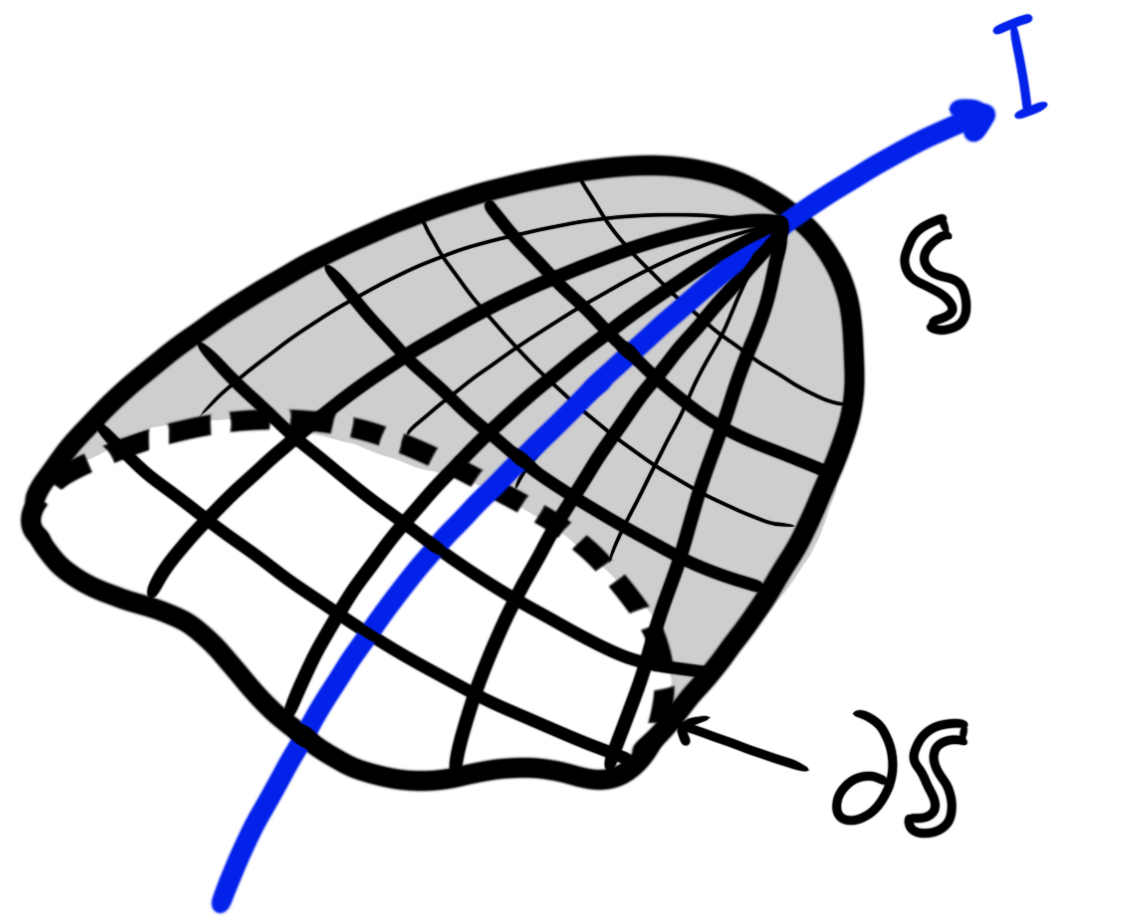
\includegraphics[width=0.5\textwidth]{im/66.png}
\end{center}

Где $I$ - полный ток через поверхность $S$. 
 
\begin{gather*}
    \mathrm{rot}\vec{H}=\frac{4\pi}{c}\vec{j}\Rightarrow \underset{S}{\iint}\mathrm{rot}\vec{H}\cdot d\vec{S}=\frac{4\pi}{c}\iint \vec{j}\cdot d\vec{S}  \\
    \Downarrow \\
    \boxed{\underset{\delta S}{\oint}\vec{H}d\vec{l}=\frac{4\pi}{c}I }\textit{ - циркуляция}
\end{gather*}

\begin{gather*}
    \mathrm{div}\vec{H}=0\Rightarrow \ \underset{V}{\iiint}\mathrm{div}\vec{H}dV=0=\underset{\delta V}{\oiint}\vec{H}d\vec{S}(\text{так как}\forall V) \\
    \Downarrow \\
    \boxed{\oiint \vec{H}d\vec{S}=0}\textit{ - поток}
\end{gather*}

\newpage

\subsection*{Граничные условия}

\begin{minipage}[c]{0.5\textwidth} % Левая часть: изображение
    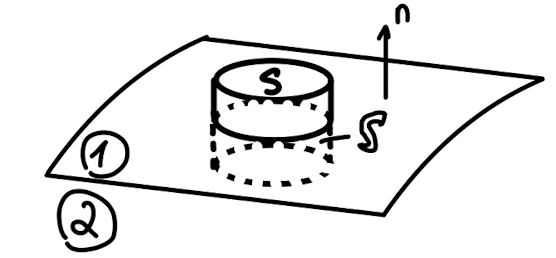
\includegraphics[width=\textwidth]{im/67.png} % Ваше изображение
\end{minipage}%
\hfill
\begin{minipage}[c]{0.55\textwidth} % Правая часть: текст
    \begin{gather*}
        \oiint \vec{H}d\vec{S}=0 \\
        H_{1n}|\cdot S-H_{2n}|\cdot S=0 \\
        \Downarrow \\
        \boxed{H_{1n}=H_{2n}} \text{ - то есть } H_n \text{ - непр.}
    \end{gather*}
\end{minipage}
\( \text{ } \)  
\begin{minipage}[c]{0.5\textwidth} % Левая часть: изображение
    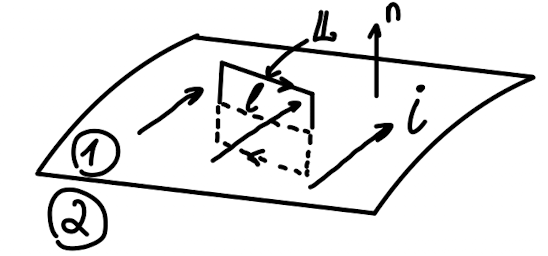
\includegraphics[width=\textwidth]{im/68.png} % Ваше изображение
\end{minipage}%
\hfill
\begin{minipage}[c]{0.55\textwidth} % Правая часть: текст
    \begin{gather*}
        \underset{L}{\oint}\vec{H}d\vec{l}=\frac{4\pi}{c}I \\
        H_{1\tau}\cdot l - H_{2\tau}\cdot l =\frac{4\pi}{c}il \\
        \Downarrow \\
        \boxed{H_{1\tau}- H_{2\tau} = \frac{4\pi}{c}i }
    \end{gather*}
\end{minipage}


